\subsection{System Dynamics}
\label{sec:sysdyn}
\subsubsection{Electrical Grid}

To begin the design, dynamics of electrical grids need to be understood, specifically how supply and demand feed into the frequency.
Supplementing this is how Maui has a {peak demand of 195MW, a yearly energy usage of 1200GWh}, 55,301 residential and 9,356 commercial customers. \cite{power:maui}.
This sizable demand means large fluctuations in the net power in the grid will occur, so an accurate model is needed.

It was observed that a net-positive power in the system causes an increase in the frequency as the energy generated \emph{must} go somewhere due to conservation of energy.
The place the energy goes is the angular momentum of the rotating masses.
The inverse is true for net-negative powers, a decrease in frequency results.

To begin tackling this problem, it is possible to consider the grid like a flywheel as suggested by \cite{power:swing}.
The governing equation is known as the \emph{Swing Equation}, which models the electrical powers of every component as a \emph{torque} on a flywheel.
This method makes sense, as the grid has an inertia associated with it, which is the rotational inertia of all power sources and sinks.

The inertia of the grid does vary with time - however for simplicity a time-invariant inertia $J$, (the inertia of my plant) is assumed.
Grid inertia has a trend of decreasing with time, consumers are following a trend of moving away from bulky, solid-core transformers which offer an inertial component, to a low-inertia switch-mode power supplies \cite{power:vi}.
This makes the control task more challenging as this will cause an increase in bandwidth of the system - by assuming a worst-case scenario of $J \approx J_{\text{plant}}$ should suffice since $J$ will be tune-able with a \emph{virtual inertia}, in Section \ref{sec:vi}.

To begin, the \emph{Swing Equation} as suggested by \cite{power:swing} was considered:
%
\begin{equation}
    P = T\omega
\end{equation}
%
\begin{equation}
        T = \frac{\partial}{\partial t} ( J \omega) = J \dot \omega
        \label{swing}
\end{equation}
%
\begin{equation}
        \therefore \qquad \dot \omega = \frac{P_{\text{net}}}{J \omega} = \frac{T_{\text{net}}}{J}, \quad \text{where} \quad  T_i = P_i \bar \omega^{-1}
\end{equation}
%
This derivation assumed an operating point $\bar \omega = 120\pi$, as that is the grid's angular frequency of the proposed location and it is not expected to deviate much from it.
The implication of this result is that a low inertia on the grid will cause \emph{large} frequency rate of change for power mismatch.

\subsubsection{Generation and Consumption Units}

Since it was already known that each component's contribution can be written as $T_i = P_i \bar \omega$, power can also be interpreted as a torque.
For an initial design a first-order response from each component was assumed, with step responses like:
\begin{equation}
        T_i(t) = T_{\text{max}_i}(1 - \mathrm{e}^{-k_i t})
\end{equation}
Which implies a transfer function:
\begin{equation}
        \overline{G_{i}(s)} = \frac{\overline{T_{i}(s)}}{\overline{U_{i}(s)}} = \frac{T_{\text{max}_{i}}k_i}{k_i + {s}}
\end{equation}

The rise times can be assumed as $\frac{3}{t_{\text{rise}_i}} \approx k_i$ as this gives an error of $\mathrm{e}^{-3}$. If this is applied through to components, a set of parameters for the model (Table \ref{tbl:powercomp}) can be generated.


%
    \begin{table}[ht]
    \label{tbl:powercomp}
            \centering
        \begin{tabular}{||l l l l l l||}
                \hline
                Component & $t_{\text{rise}}$ & $k$ / s$^{-1}$ & $\eta_{\text{therm}}$ & $P_{\text{max}}$/MW& Minimum Use / \%\\
                \hline
                \hline
                Turbine& 8 mins & 0.375 & 0.65 & 250MW & 10\\
                \hline
                SOFC& 35 mins & 0.0857 & 0.90 & 230MW & 30\\
                \hline
                Electrolyser& 80 seconds & 2.25 & N/A & 300MW & 20\\
                \hline
                Cryo-Still & 40 mins & 4.50 & N/A & - & 30\\
                \hline
        \end{tabular}
        \caption{A table to capture the properties of the many systems in the ESS}
                \label{tbl:time}
    \end{table}

\subsubsection{Modelling Wind Power}

As specified in the project brief, the only allowed power source are wind turbines.
Wind turbines offer the ability to generate a lot of clean energy, but are very intermittent in their supply.
For this design to be more accurate, a good model on how wind speed correlates with power generated was developed.

The wind turbine `GE Haliade-150-6MW' was chosen as a good candidate, as it offers offshore 6MW generation, is domestic to the US market and has better specifications to its competitors.
As suggested by \cite{power:wturbine}, a reasonable approximation to the turbine model was found by considering a double-exponential model, which is of form:
%
\begin{equation}
        \label{eqn:wturbexm}
        P_{\text{gen}} =
        \begin{cases}
                P_{\text{rated}} \exp ( -\tau_1 \exp (-v \tau_2)),& 0 \leq v < v_{\text{cutout}}\\
                0,& v_{\text{cutout}} \leq v
        \end{cases}
\end{equation}

The wind turbine's `cut-in' speed is known, this is the speed at which the turbine begins to generate electricity.
Also known is the `rated speed', the speed at which the turbine generates maximum power.
An \emph{iterative convergent scheme} was setup in MATLAB (using gradient descent), and used the information in Table \ref{tbl:haliade} to build the model and obtain time constants $\tau_1 = 70.9780,\tau_2 = 0.7130$.
%
\begin{table}[bh]
        \centering
        \begin{tabular}{||l | l||}
                \hline
                $P_{\text{rated}}$ & $6000kW$\\
                \hline
                $v_{\text{cutin}}$ & $3ms^{-1}$\\
                \hline
                $v_{\text{cutout}}$ & $25ms^{-1}$\\
                \hline
                $v_{\text{rated}}$ & $12.5ms^{-1}$\\
                \hline
        \end{tabular}
        \caption{GE Haliade-150-6MW data from GE datasheet and private communication. \cite{power:wturbdata}} \label{tbl:haliade}
\end{table}

Using the obtained constants, the characteristic steady-state power curve for the wind turbine can be plotted, as shown in Figure \ref{fig:wturb}.
By assuming that the turbine is always at steady state, it is easy to see estimating the wind power is a relatively simple task, by injecting windspeed in and multiply the result by the number of turbines in the field.

The NOAA supply historical data on hourly wind-speeds \cite{power:NOAA}, as well as predicted future wind-speeds.
This historical data-set was used to validate our model by considering how real-world wind-speed works with energy generation.
Using Equation \ref{eqn:wturbexm} and using $\tau_1, \tau_2$ the yearly generated energy in Maui can be plotted.
           \begin{figure}[bht]
                   \centering
                   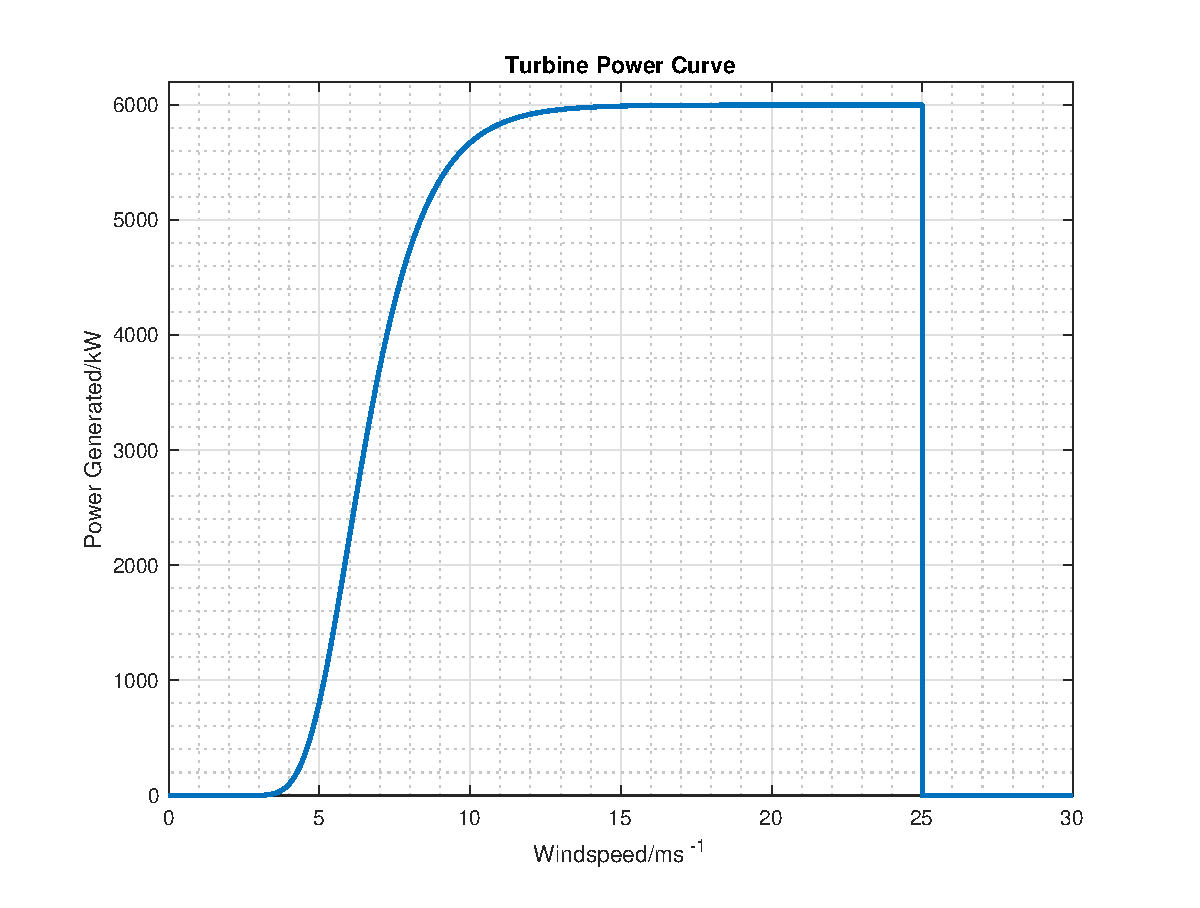
\includegraphics[scale=0.4]{./images/turbine.eps}
                   \caption{Approximated Steady State Power Response of the GE Haliade-150-6MW} \label{fig:wturb}
           \end{figure}

Equation \ref{eqn:wturbexm} was applied to the wind speed data-set with 65 turbines, to obtain the power data below in Figure \ref{fig:speedpowermap}.

The data obtained had values for every fifteen minutes, which although is a high resolution, a cubic spline fit gives an approximation on the second-by-second level.
This is an approximation to what reality is with windspeed, however since turbine transfer functions for dynamic cases were not considered - this may make a good approximation to reality.

Similarly for demand, the EIA supply data sets for electrical demand \cite{power:EIA}, which were smoothed with cubic splines and cleaned for use later.

\begin{figure}[t]
\centering
\begin{subfigure}{.5\textwidth}
  \centering
  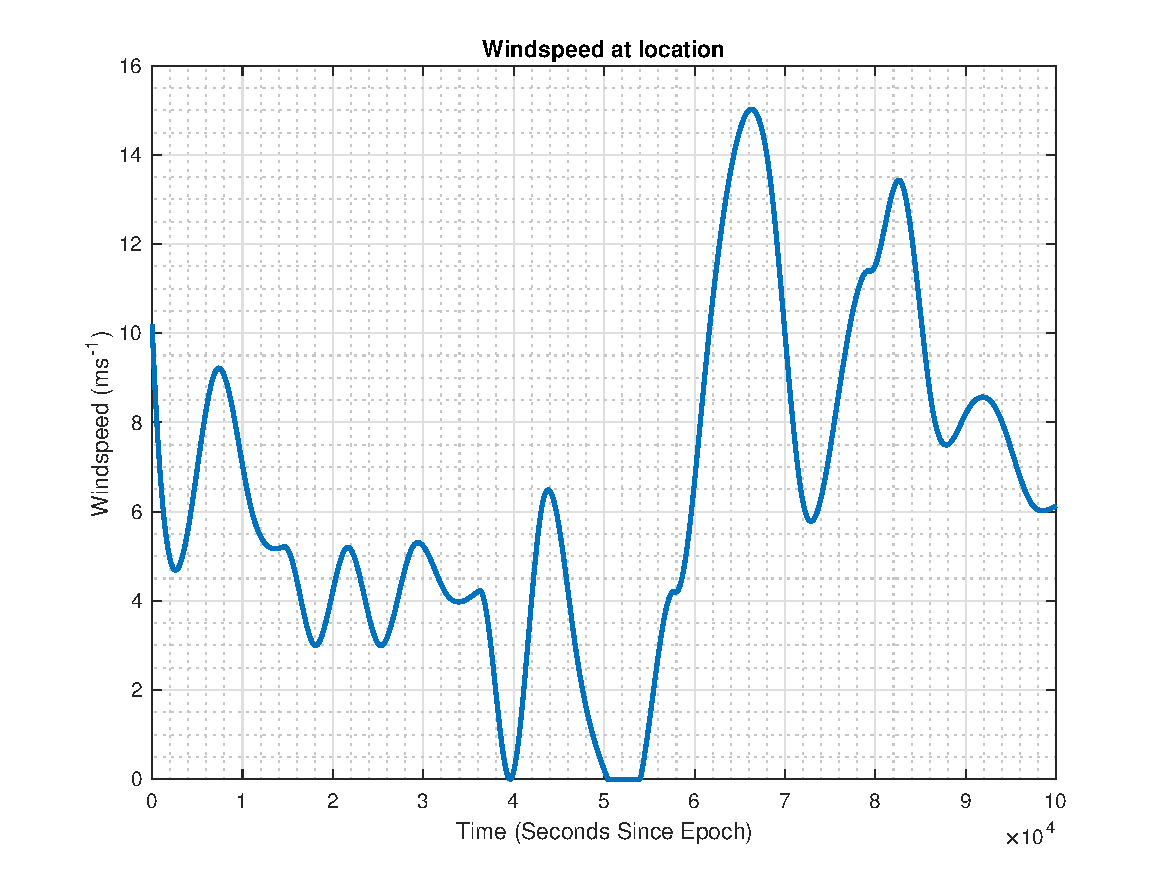
\includegraphics[scale=0.4]{./images/AWindspeed-eps-converted-to.pdf}
  \caption{Windspeed in Maui}
  \label{fig:windspeed}
\end{subfigure}%
\begin{subfigure}{.5\textwidth}
  \centering
  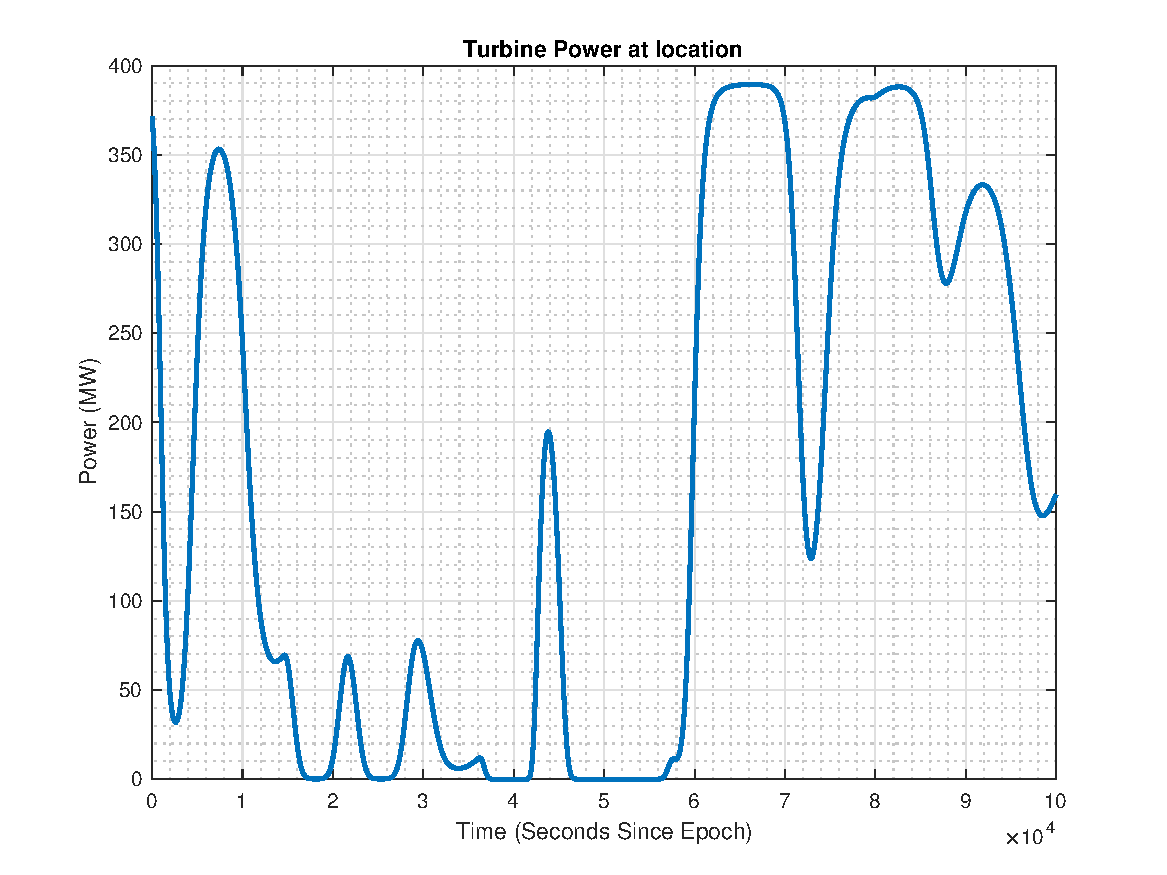
\includegraphics[scale=0.4]{./images/AWindpower-eps-converted-to.pdf}
  \caption{Electrical Power Obtained from 65 Wind Turbines}
  \label{fig:windpower}
\end{subfigure}
        \caption{Windspeed Mapping to Electrical Power by Applying Equation \ref{eqn:wturbexm} Over the First $10^5$ Seconds of Data}
\label{fig:speedpowermap}
\end{figure}
